\SourceLeaf{240}%
\par
Dann ist:

\[
\text{Volumen } ABCabc = \tfrac{1}{2}\, Aa \cdot BC \cdot \frac{\sin iAD}{i}.
\]


Noch zierlicher: Inhalt der Pyramide $ABCD$ [, bei welcher der Winkel $ABC$
$= 90^0$ und ein] unendlich kleiner diedrischer Winkel an $AB = \theta$.

\begin{center}
\begin{minipage}[b]{6.1cm}\begin{center}
$AB = x,$

$AC = r.$

Volumen $= \tfrac{1}{2}(x - r\cos\varphi)\,.\,\theta.$
\end{center}\end{minipage}\hfill
\begin{minipage}[b]{6.5cm}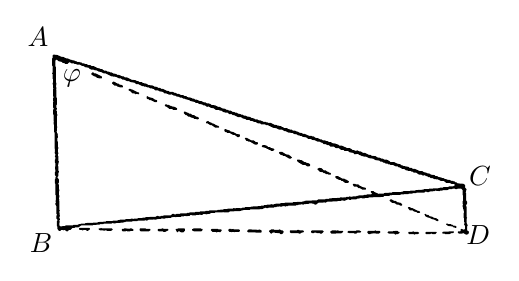
\begin{tikzpicture}[x=0.00615530cm,y=-0.00615530cm]
\fill[even odd rule] (860,458) -- (862,460) -- (870,460) -- (871,459) -- (874,459) -- (875,460) -- (880,460) -- (883,457) -- (883,456) -- (882,455) -- (862,455) -- (860,457) -- cycle
(919,455) -- (918,454) -- (896,455) -- (895,456) -- (895,458) -- (896,459) -- (900,459) -- (901,460) -- (909,460) -- (913,458) -- (917,458) -- (919,456) -- cycle
(825,456) -- (825,458) -- (827,460) -- (836,460) -- (837,461) -- (839,460) -- (844,460) -- (847,458) -- (847,457) -- (844,455) -- (836,455) -- (835,454) -- (833,455) -- (826,455) -- cycle
(782,456) -- (782,457) -- (785,459) -- (796,459) -- (798,461) -- (800,460) -- (803,460) -- (807,457) -- (806,455) -- (804,455) -- (802,453) -- (798,453) -- (797,454) -- (795,453) -- (793,454) -- (784,454) -- cycle
(767,455) -- (765,453) -- (758,453) -- (757,452) -- (755,453) -- (742,453) -- (740,455) -- (740,457) -- (743,460) -- (746,460) -- (747,459) -- (750,459) -- (751,458) -- (763,459) -- (765,458) -- (767,456) -- cycle
(727,454) -- (723,452) -- (718,452) -- (717,453) -- (702,453) -- (700,454) -- (699,456) -- (703,458) -- (713,458) -- (714,459) -- (717,459) -- (719,457) -- (725,457) -- (727,455) -- cycle
(664,457) -- (666,459) -- (687,458) -- (690,455) -- (690,454) -- (689,453) -- (681,453) -- (680,452) -- (678,452) -- (677,453) -- (675,452) -- (668,452) -- (664,454) -- cycle
(624,454) -- (624,456) -- (626,458) -- (629,458) -- (630,457) -- (635,457) -- (636,458) -- (642,458) -- (643,459) -- (646,459) -- (650,455) -- (650,454) -- (647,452) -- (626,452) -- cycle
(609,454) -- (607,452) -- (600,452) -- (599,451) -- (596,451) -- (595,452) -- (581,452) -- (580,453) -- (580,456) -- (583,458) -- (598,458) -- (599,459) -- (601,459) -- (604,457) -- (608,456) -- cycle
(537,453) -- (537,454) -- (541,459) -- (542,459) -- (544,457) -- (548,456) -- (549,457) -- (559,458) -- (561,460) -- (563,460) -- (565,459) -- (567,456) -- (567,454) -- (565,452) -- (562,452) -- (559,450) -- (557,451) -- (548,451) -- (547,450) -- (542,450) -- cycle
(492,453) -- (492,454) -- (494,456) -- (509,456) -- (510,457) -- (520,457) -- (522,455) -- (522,453) -- (520,451) -- (518,451) -- (517,450) -- (515,451) -- (495,450) -- cycle
(453,451) -- (453,453) -- (455,455) -- (459,455) -- (460,456) -- (462,455) -- (464,455) -- (465,456) -- (467,455) -- (475,455) -- (477,453) -- (477,452) -- (475,450) -- (464,450) -- (463,449) -- (460,450) -- (459,449) -- (455,449) -- cycle
(417,451) -- (417,452) -- (420,455) -- (427,455) -- (428,456) -- (430,456) -- (431,455) -- (436,456) -- (439,453) -- (439,451) -- (438,450) -- (432,450) -- (431,449) -- (419,449) -- cycle
(378,450) -- (378,452) -- (382,454) -- (397,454) -- (400,451) -- (399,449) -- (397,449) -- (396,448) -- (382,448) -- cycle
(344,450) -- (347,456) -- (348,456) -- (350,454) -- (352,454) -- (355,456) -- (360,456) -- (363,453) -- (363,449) -- (362,448) -- (349,448) -- (348,449) -- (345,449) -- cycle
(307,451) -- (307,452) -- (309,454) -- (318,454) -- (319,455) -- (323,455) -- (329,452) -- (329,450) -- (328,449) -- (319,449) -- (318,448) -- (316,448) -- (315,449) -- (309,449) -- cycle
(270,449) -- (270,452) -- (272,454) -- (289,454) -- (292,452) -- (292,450) -- (291,449) -- (283,449) -- (282,448) -- (271,448) -- cycle
(233,450) -- (233,452) -- (235,454) -- (241,454) -- (242,453) -- (244,454) -- (250,454) -- (251,453) -- (256,453) -- (257,452) -- (257,450) -- (253,448) -- (250,448) -- (249,449) -- (247,449) -- (246,448) -- (244,449) -- (242,448) -- (238,448) -- (237,449) -- (234,449) -- cycle
(185,449) -- (185,450) -- (188,452) -- (195,452) -- (196,453) -- (198,452) -- (201,452) -- (202,453) -- (211,453) -- (214,451) -- (214,450) -- (212,448) -- (192,448) -- (190,447) -- (189,448) -- (186,448) -- cycle
(145,448) -- (145,450) -- (146,451) -- (150,451) -- (151,452) -- (153,452) -- (154,451) -- (158,451) -- (161,453) -- (163,453) -- (167,450) -- (167,448) -- (166,447) -- (146,447) -- cycle
(903,439) -- (903,440) -- (907,443) -- (916,444) -- (918,446) -- (920,446) -- (921,447) -- (923,447) -- (924,446) -- (924,444) -- (923,443) -- (917,442) -- (915,440) -- (913,440) -- (912,439) -- (907,439) -- (906,438) -- (904,438) -- cycle
(858,419) -- (860,423) -- (866,426) -- (868,426) -- (874,429) -- (879,430) -- (884,433) -- (886,433) -- (887,432) -- (887,430) -- (882,427) -- (877,426) -- (875,424) -- (873,424) -- (872,423) -- (869,423) -- (866,420) -- (863,420) -- (860,418) -- cycle
(824,405) -- (824,406) -- (828,411) -- (834,411) -- (836,413) -- (841,414) -- (844,416) -- (848,416) -- (849,415) -- (849,414) -- (847,412) -- (845,412) -- (833,406) -- (831,406) -- (827,404) -- (825,404) -- cycle
(786,390) -- (786,391) -- (791,395) -- (797,396) -- (801,399) -- (805,399) -- (808,401) -- (811,401) -- (812,400) -- (812,398) -- (808,395) -- (802,394) -- (798,391) -- (795,391) -- (790,388) -- (788,388) -- cycle
(90,91) -- (90,96) -- (89,97) -- (89,111) -- (91,115) -- (90,116) -- (90,126) -- (89,128) -- (90,129) -- (90,139) -- (91,140) -- (91,147) -- (90,148) -- (90,150) -- (91,151) -- (91,158) -- (92,159) -- (91,161) -- (91,175) -- (92,176) -- (92,178) -- (91,179) -- (91,185) -- (92,186) -- (91,188) -- (91,198) -- (92,199) -- (92,202) -- (91,203) -- (91,212) -- (92,213) -- (92,226) -- (93,227) -- (92,229) -- (92,233) -- (93,234) -- (93,249) -- (94,250) -- (94,283) -- (95,284) -- (95,290) -- (94,292) -- (96,295) -- (96,297) -- (95,298) -- (95,300) -- (96,301) -- (96,305) -- (95,306) -- (95,312) -- (96,313) -- (96,320) -- (95,321) -- (96,331) -- (95,332) -- (95,338) -- (97,341) -- (96,343) -- (96,346) -- (95,347) -- (95,355) -- (96,356) -- (96,379) -- (97,380) -- (97,390) -- (96,391) -- (97,395) -- (96,396) -- (96,399) -- (98,402) -- (98,418) -- (99,419) -- (99,421) -- (98,422) -- (98,428) -- (100,430) -- (100,432) -- (99,433) -- (99,443) -- (100,444) -- (100,449) -- (103,453) -- (106,453) -- (108,451) -- (111,451) -- (112,452) -- (115,451) -- (119,454) -- (121,454) -- (124,451) -- (127,451) -- (131,447) -- (135,447) -- (136,446) -- (143,446) -- (149,442) -- (173,442) -- (174,441) -- (187,440) -- (188,439) -- (195,439) -- (196,438) -- (212,438) -- (213,437) -- (219,438) -- (220,437) -- (236,436) -- (237,435) -- (240,435) -- (241,434) -- (254,434) -- (255,433) -- (265,433) -- (266,432) -- (280,432) -- (281,431) -- (285,432) -- (288,430) -- (298,430) -- (299,429) -- (301,430) -- (304,430) -- (305,429) -- (315,428) -- (316,427) -- (318,428) -- (322,428) -- (323,427) -- (335,426) -- (336,425) -- (339,425) -- (340,424) -- (345,425) -- (346,424) -- (355,424) -- (356,423) -- (361,423) -- (362,422) -- (368,423) -- (369,422) -- (373,422) -- (375,420) -- (377,420) -- (378,421) -- (386,421) -- (387,420) -- (393,420) -- (394,419) -- (396,420) -- (399,420) -- (402,418) -- (409,419) -- (410,418) -- (414,418) -- (418,416) -- (425,416) -- (426,415) -- (441,415) -- (442,414) -- (444,415) -- (453,415) -- (456,413) -- (479,412) -- (480,411) -- (483,411) -- (484,410) -- (497,410) -- (498,409) -- (517,409) -- (518,408) -- (523,408) -- (530,405) -- (532,406) -- (535,406) -- (536,405) -- (547,405) -- (548,404) -- (552,404) -- (553,403) -- (557,403) -- (558,402) -- (560,403) -- (564,403) -- (565,402) -- (569,402) -- (571,403) -- (572,402) -- (576,402) -- (577,401) -- (592,401) -- (593,400) -- (597,400) -- (598,399) -- (602,399) -- (603,398) -- (608,399) -- (609,398) -- (620,397) -- (621,396) -- (629,397) -- (632,399) -- (634,399) -- (639,395) -- (649,395) -- (650,394) -- (654,395) -- (657,393) -- (678,392) -- (679,391) -- (686,391) -- (687,390) -- (693,391) -- (700,388) -- (702,388) -- (703,389) -- (706,389) -- (707,388) -- (717,388) -- (720,386) -- (721,387) -- (722,386) -- (725,386) -- (726,385) -- (728,385) -- (729,386) -- (734,386) -- (735,385) -- (742,385) -- (743,384) -- (773,383) -- (775,381) -- (785,381) -- (787,379) -- (789,380) -- (791,379) -- (808,379) -- (809,378) -- (815,378) -- (816,377) -- (825,377) -- (826,376) -- (833,376) -- (834,375) -- (841,375) -- (842,374) -- (858,374) -- (860,372) -- (862,372) -- (863,373) -- (867,373) -- (868,372) -- (879,371) -- (880,370) -- (889,371) -- (890,370) -- (895,370) -- (896,369) -- (905,369) -- (909,367) -- (915,367) -- (916,366) -- (921,366) -- (922,367) -- (925,367) -- (926,366) -- (934,366) -- (937,369) -- (937,379) -- (938,380) -- (938,391) -- (937,392) -- (937,397) -- (938,399) -- (937,400) -- (937,404) -- (938,405) -- (938,408) -- (939,409) -- (939,412) -- (940,413) -- (940,415) -- (939,416) -- (939,426) -- (940,427) -- (940,435) -- (941,436) -- (940,440) -- (942,443) -- (942,449) -- (940,451) -- (934,449) -- (933,450) -- (933,453) -- (932,454) -- (928,454) -- (927,455) -- (927,457) -- (930,459) -- (936,459) -- (937,458) -- (939,458) -- (944,461) -- (948,460) -- (949,459) -- (950,455) -- (946,452) -- (946,444) -- (947,443) -- (947,441) -- (945,437) -- (945,428) -- (946,426) -- (945,425) -- (945,403) -- (944,402) -- (944,400) -- (946,397) -- (946,393) -- (944,390) -- (944,375) -- (943,374) -- (945,367) -- (942,364) -- (942,359) -- (939,356) -- (926,355) -- (924,353) -- (922,353) -- (920,351) -- (918,351) -- (917,350) -- (914,350) -- (910,348) -- (906,348) -- (905,347) -- (900,346) -- (897,344) -- (894,344) -- (893,343) -- (887,342) -- (884,340) -- (881,340) -- (879,338) -- (871,337) -- (869,335) -- (863,334) -- (862,333) -- (857,332) -- (854,330) -- (849,330) -- (838,325) -- (834,325) -- (831,323) -- (827,323) -- (825,321) -- (814,319) -- (813,318) -- (811,318) -- (809,316) -- (801,314) -- (795,311) -- (788,311) -- (786,309) -- (780,306) -- (775,306) -- (772,304) -- (769,304) -- (765,302) -- (762,302) -- (757,299) -- (749,298) -- (746,296) -- (743,296) -- (735,292) -- (731,292) -- (726,289) -- (723,289) -- (720,287) -- (715,288) -- (714,287) -- (709,286) -- (707,284) -- (703,282) -- (698,282) -- (687,277) -- (682,277) -- (680,275) -- (676,274) -- (675,273) -- (667,272) -- (665,270) -- (661,270) -- (658,268) -- (656,268) -- (652,266) -- (648,266) -- (645,264) -- (642,264) -- (639,262) -- (633,261) -- (629,258) -- (626,258) -- (625,257) -- (620,257) -- (611,253) -- (608,253) -- (604,251) -- (601,251) -- (596,248) -- (594,248) -- (590,246) -- (586,246) -- (584,244) -- (580,244) -- (579,243) -- (577,243) -- (574,241) -- (568,241) -- (566,239) -- (564,239) -- (562,237) -- (559,237) -- (558,236) -- (555,236) -- (551,234) -- (548,234) -- (540,230) -- (535,230) -- (534,229) -- (531,229) -- (530,228) -- (526,228) -- (519,225) -- (516,225) -- (513,223) -- (508,223) -- (506,221) -- (501,220) -- (498,218) -- (492,217) -- (488,215) -- (485,215) -- (482,213) -- (479,213) -- (478,212) -- (473,211) -- (470,209) -- (467,209) -- (466,208) -- (461,207) -- (458,205) -- (454,205) -- (452,203) -- (449,203) -- (446,201) -- (440,200) -- (435,197) -- (432,197) -- (426,194) -- (418,193) -- (416,191) -- (414,191) -- (413,190) -- (409,190) -- (406,188) -- (403,188) -- (397,185) -- (394,185) -- (387,182) -- (384,182) -- (382,180) -- (379,180) -- (375,178) -- (368,177) -- (366,175) -- (363,175) -- (360,173) -- (356,173) -- (350,170) -- (347,170) -- (344,168) -- (342,168) -- (338,166) -- (332,166) -- (329,164) -- (326,164) -- (318,160) -- (315,160) -- (312,158) -- (308,158) -- (306,156) -- (300,155) -- (297,153) -- (288,152) -- (283,149) -- (277,148) -- (274,146) -- (270,146) -- (267,144) -- (265,144) -- (261,142) -- (253,141) -- (243,136) -- (239,136) -- (237,134) -- (234,134) -- (227,131) -- (224,131) -- (221,129) -- (215,128) -- (212,126) -- (209,126) -- (206,124) -- (203,124) -- (200,122) -- (196,122) -- (192,119) -- (189,119) -- (188,118) -- (183,117) -- (175,113) -- (171,113) -- (168,111) -- (164,111) -- (161,109) -- (158,109) -- (154,107) -- (151,107) -- (149,105) -- (146,105) -- (145,104) -- (142,105) -- (140,103) -- (138,103) -- (134,101) -- (131,101) -- (130,100) -- (128,100) -- (121,97) -- (118,97) -- (112,94) -- (109,94) -- (100,90) -- (92,89) -- cycle
(96,101) -- (98,99) -- (103,103) -- (109,104) -- (111,106) -- (115,107) -- (116,108) -- (121,108) -- (124,105) -- (126,105) -- (129,107) -- (134,107) -- (135,108) -- (138,108) -- (141,110) -- (147,110) -- (150,112) -- (155,113) -- (157,115) -- (164,116) -- (166,118) -- (170,120) -- (175,120) -- (176,121) -- (182,122) -- (185,124) -- (190,125) -- (196,128) -- (200,128) -- (212,134) -- (221,135) -- (227,138) -- (231,138) -- (235,141) -- (238,141) -- (244,144) -- (248,144) -- (252,146) -- (259,147) -- (263,150) -- (267,150) -- (275,154) -- (278,154) -- (279,155) -- (282,155) -- (286,157) -- (289,157) -- (292,159) -- (296,159) -- (297,160) -- (299,160) -- (302,163) -- (308,163) -- (311,165) -- (318,166) -- (321,169) -- (325,169) -- (326,170) -- (328,170) -- (330,172) -- (334,172) -- (336,171) -- (341,174) -- (344,174) -- (347,176) -- (350,176) -- (354,178) -- (357,178) -- (360,180) -- (363,180) -- (364,181) -- (372,183) -- (375,185) -- (384,187) -- (386,189) -- (390,189) -- (393,191) -- (399,192) -- (402,194) -- (405,194) -- (409,197) -- (412,196) -- (417,199) -- (423,200) -- (427,203) -- (433,203) -- (436,205) -- (439,205) -- (443,208) -- (445,208) -- (446,209) -- (452,209) -- (455,212) -- (460,212) -- (462,214) -- (465,214) -- (473,218) -- (479,218) -- (483,221) -- (488,222) -- (491,224) -- (496,224) -- (499,226) -- (502,226) -- (506,228) -- (509,228) -- (514,231) -- (519,231) -- (521,233) -- (529,233) -- (531,235) -- (535,235) -- (545,240) -- (552,241) -- (558,244) -- (564,244) -- (569,247) -- (571,247) -- (577,250) -- (586,251) -- (589,253) -- (595,254) -- (597,256) -- (600,256) -- (601,257) -- (604,257) -- (607,259) -- (614,260) -- (618,263) -- (623,263) -- (626,265) -- (632,266) -- (638,269) -- (642,269) -- (645,271) -- (647,271) -- (650,274) -- (654,274) -- (658,276) -- (661,276) -- (664,279) -- (671,279) -- (675,282) -- (681,282) -- (686,286) -- (691,286) -- (693,288) -- (700,288) -- (704,291) -- (711,292) -- (714,295) -- (720,294) -- (725,297) -- (727,297) -- (729,299) -- (732,299) -- (733,300) -- (738,300) -- (744,303) -- (752,304) -- (757,307) -- (765,308) -- (767,310) -- (771,310) -- (773,312) -- (775,312) -- (778,314) -- (782,314) -- (784,316) -- (787,316) -- (788,317) -- (793,317) -- (799,320) -- (803,320) -- (805,322) -- (807,322) -- (812,325) -- (816,325) -- (820,328) -- (823,328) -- (824,329) -- (829,329) -- (832,331) -- (834,331) -- (836,333) -- (841,333) -- (847,337) -- (852,337) -- (855,339) -- (859,338) -- (861,340) -- (864,340) -- (866,342) -- (869,342) -- (871,344) -- (875,344) -- (878,346) -- (886,347) -- (892,350) -- (898,350) -- (903,354) -- (910,354) -- (914,356) -- (919,356) -- (921,358) -- (921,359) -- (918,361) -- (909,361) -- (907,363) -- (897,363) -- (896,364) -- (890,364) -- (889,365) -- (868,366) -- (867,367) -- (857,367) -- (856,368) -- (840,369) -- (839,370) -- (829,370) -- (828,371) -- (815,371) -- (814,372) -- (811,372) -- (810,373) -- (792,373) -- (791,374) -- (775,375) -- (774,376) -- (765,376) -- (764,377) -- (755,373) -- (753,371) -- (748,371) -- (747,373) -- (750,376) -- (748,378) -- (739,378) -- (738,379) -- (733,379) -- (732,380) -- (722,380) -- (721,381) -- (718,381) -- (717,382) -- (710,382) -- (709,383) -- (703,382) -- (702,383) -- (697,383) -- (696,384) -- (691,384) -- (690,385) -- (688,384) -- (684,384) -- (683,385) -- (662,386) -- (661,387) -- (654,387) -- (653,388) -- (639,388) -- (636,390) -- (611,391) -- (610,392) -- (607,392) -- (606,393) -- (595,393) -- (594,394) -- (587,394) -- (586,395) -- (570,395) -- (569,396) -- (561,396) -- (560,397) -- (551,397) -- (550,398) -- (547,398) -- (546,399) -- (541,398) -- (540,399) -- (533,399) -- (532,400) -- (527,400) -- (526,401) -- (521,401) -- (520,402) -- (500,403) -- (499,404) -- (488,404) -- (487,405) -- (483,405) -- (479,407) -- (477,406) -- (469,406) -- (468,407) -- (464,406) -- (463,407) -- (452,407) -- (451,408) -- (444,408) -- (443,409) -- (431,410) -- (430,411) -- (414,411) -- (413,412) -- (406,412) -- (405,413) -- (395,413) -- (394,414) -- (385,414) -- (384,415) -- (373,415) -- (372,416) -- (368,416) -- (367,417) -- (354,417) -- (353,418) -- (346,418) -- (345,419) -- (341,419) -- (340,418) -- (338,418) -- (334,421) -- (320,421) -- (319,422) -- (314,422) -- (313,423) -- (309,423) -- (307,422) -- (303,424) -- (291,424) -- (290,425) -- (282,425) -- (281,426) -- (276,426) -- (275,427) -- (266,427) -- (265,428) -- (258,428) -- (257,429) -- (255,428) -- (252,428) -- (251,429) -- (241,429) -- (240,430) -- (229,430) -- (228,431) -- (225,431) -- (224,432) -- (215,432) -- (214,433) -- (201,433) -- (200,434) -- (184,435) -- (183,436) -- (158,437) -- (157,438) -- (149,438) -- (148,439) -- (145,439) -- (141,441) -- (133,441) -- (132,442) -- (117,442) -- (116,443) -- (106,444) -- (104,442) -- (104,436) -- (105,435) -- (104,433) -- (104,431) -- (105,430) -- (105,428) -- (104,427) -- (104,424) -- (105,423) -- (104,413) -- (105,411) -- (104,410) -- (104,392) -- (103,391) -- (104,389) -- (103,387) -- (103,385) -- (104,384) -- (104,380) -- (103,379) -- (103,372) -- (104,371) -- (104,368) -- (103,367) -- (103,358) -- (102,357) -- (102,354) -- (103,353) -- (103,347) -- (100,343) -- (100,342) -- (102,340) -- (102,333) -- (103,332) -- (103,330) -- (102,329) -- (102,320) -- (101,319) -- (103,310) -- (102,309) -- (102,299) -- (101,298) -- (101,295) -- (102,294) -- (102,292) -- (101,291) -- (101,284) -- (102,283) -- (102,281) -- (101,280) -- (101,269) -- (100,268) -- (100,261) -- (101,260) -- (101,257) -- (100,255) -- (101,253) -- (99,251) -- (99,249) -- (98,248) -- (99,246) -- (99,240) -- (100,239) -- (99,237) -- (99,216) -- (100,215) -- (100,213) -- (99,212) -- (99,206) -- (98,205) -- (98,203) -- (99,202) -- (99,200) -- (98,199) -- (98,193) -- (99,192) -- (99,179) -- (98,178) -- (98,163) -- (97,162) -- (98,160) -- (98,157) -- (97,156) -- (98,148) -- (97,147) -- (97,115) -- (96,114) -- cycle
(710,357) -- (712,361) -- (714,362) -- (719,362) -- (722,365) -- (725,365) -- (730,368) -- (736,368) -- (737,367) -- (737,365) -- (736,364) -- (731,363) -- (723,359) -- (721,357) -- (716,357) -- (715,356) -- (711,356) -- cycle
(674,341) -- (674,343) -- (676,345) -- (682,348) -- (685,348) -- (687,350) -- (689,350) -- (694,354) -- (700,354) -- (702,352) -- (702,351) -- (700,349) -- (698,349) -- (696,347) -- (694,347) -- (692,345) -- (688,345) -- (679,340) -- (675,340) -- cycle
(637,325) -- (637,326) -- (642,331) -- (648,332) -- (650,334) -- (653,334) -- (655,336) -- (659,336) -- (660,337) -- (664,337) -- (665,336) -- (665,335) -- (663,333) -- (661,333) -- (659,331) -- (657,331) -- (654,328) -- (650,328) -- (646,324) -- (641,323) -- cycle
(595,307) -- (595,309) -- (597,311) -- (607,317) -- (612,317) -- (616,320) -- (620,320) -- (622,318) -- (622,316) -- (620,314) -- (613,312) -- (612,311) -- (610,311) -- (604,307) -- (601,307) -- (600,306) -- (596,306) -- cycle
(558,291) -- (558,293) -- (561,296) -- (565,297) -- (566,298) -- (569,298) -- (579,304) -- (582,304) -- (584,302) -- (584,301) -- (578,296) -- (572,295) -- (564,290) -- (559,290) -- cycle
(522,278) -- (523,280) -- (531,282) -- (533,284) -- (535,284) -- (537,286) -- (539,286) -- (542,288) -- (545,288) -- (548,286) -- (548,285) -- (546,283) -- (541,282) -- (539,280) -- (535,280) -- (532,277) -- (530,277) -- (529,276) -- (524,276) -- cycle
(487,262) -- (490,267) -- (494,268) -- (495,269) -- (498,269) -- (508,275) -- (512,275) -- (514,273) -- (514,271) -- (513,270) -- (510,270) -- (505,266) -- (500,266) -- (491,261) -- (488,261) -- cycle
(445,244) -- (445,247) -- (447,249) -- (449,249) -- (451,251) -- (456,251) -- (463,255) -- (466,255) -- (473,260) -- (477,258) -- (477,255) -- (476,254) -- (470,253) -- (463,249) -- (458,248) -- (456,246) -- (449,244) -- (448,243) -- (446,243) -- cycle
(407,228) -- (407,230) -- (408,231) -- (410,231) -- (416,235) -- (419,235) -- (426,240) -- (433,240) -- (434,239) -- (434,238) -- (432,236) -- (430,236) -- (421,231) -- (419,231) -- (417,229) -- (415,229) -- (411,226) -- cycle
(361,208) -- (361,210) -- (365,214) -- (367,214) -- (370,217) -- (373,217) -- (376,219) -- (381,220) -- (383,222) -- (387,222) -- (388,223) -- (390,223) -- (392,221) -- (392,220) -- (390,218) -- (386,217) -- (382,214) -- (379,214) -- (375,211) -- (372,211) -- (370,209) -- (368,209) -- (364,207) -- (362,207) -- cycle
(322,193) -- (322,195) -- (323,196) -- (326,197) -- (331,201) -- (336,201) -- (339,203) -- (346,203) -- (347,202) -- (347,200) -- (342,197) -- (336,196) -- (335,195) -- (333,195) -- (330,193) -- (327,193) -- (326,192) -- (323,192) -- cycle
(284,176) -- (284,179) -- (286,181) -- (288,181) -- (290,183) -- (293,183) -- (301,187) -- (305,187) -- (306,186) -- (306,184) -- (305,183) -- (301,182) -- (297,179) -- (289,177) -- (286,175) -- cycle
(247,161) -- (247,163) -- (251,165) -- (255,169) -- (259,169) -- (261,171) -- (263,170) -- (268,171) -- (269,170) -- (269,168) -- (268,167) -- (266,167) -- (254,161) -- (252,161) -- (251,160) -- (248,160) -- cycle
(213,147) -- (213,149) -- (218,153) -- (222,153) -- (224,155) -- (228,156) -- (229,157) -- (234,157) -- (235,156) -- (235,154) -- (233,152) -- (228,151) -- (226,149) -- (224,149) -- (217,145) -- (215,145) -- cycle
(170,128) -- (170,130) -- (176,134) -- (178,134) -- (182,137) -- (184,137) -- (185,138) -- (191,138) -- (192,137) -- (192,135) -- (191,134) -- (179,128) -- (176,128) -- (174,126) -- (172,126) -- cycle;
\node[inner sep=0pt] at (60,53) {$A$};
\node[inner sep=0pt] at (130,137) {$\varphi$};
\node[inner sep=0pt] at (973,340) {$C$};
\node[inner sep=0pt] at (969,462) {$D$};
\node[inner sep=0pt] at (66,479) {$B$};
\end{tikzpicture}
\end{minipage}
\end{center}

\Needspace{8\baselineskip}
\begin{center}


\textsc{Bemerkungen.}
\end{center}


\begingroup\small
Die in dem Briefe an \textsc{Encke} erwähnte Abhandlung in russischer Sprache ist
höchst wahrscheinlich die im ersten Hefte des Jahrganges 1836 der Kasaner Gelehrten
Schriften erschienene Arbeit: \gausscyr{Примѣненіе воображаемой геометріи къ нѣкоторымъ
интеграламъ} (Anwendung der imaginären Geometrie auf einige Integrale), von der sich
ein mit eigenem Titelblatte versehener Sonderabdruck in \textsc{Gauss}' Nachlass
befindet; einzelne Randbemerkungen sowie ein darin liegender Zettel, der die Notiz
[2] enthält, zeigen, dass \textsc{Gauss} in dieser Arbeit wirklich gelesen hat.


Die kleine Schrift in deutscher Sprache sind die \emph{Geometrischen Untersuchungen
zur Theorie der Parallellinien}, Berlin 1840, die in \textsc{Gersdorfs} Repertorium
der gesammten deutschen Literatur, Jahrgang 1840, Bd. 3, S. 147 besprochen wurden;
durch diese Anzeige scheint \textsc{Gauss} darauf aufmerksam geworden zu sein.


Statt \textsc{Knorre} muss es höchst wahrscheinlich \textsc{Knorr} heissen, denn der
mit \textsc{Lobatschefskij} engbefreundete Physiker \textsc{Ernst Knorr} war von 1832
bis 1846 Professor in Kasan und hat im Jahre 1840 eine längere Reise nach Westeuropa
gemacht, während der Astronom \textsc{K. F. Knorre} in Nikolajew keine Beziehungen zu
\textsc{Lobatschefskij} hatte und vor 1841 nur einmal in Deutschland gewesen ist, ohne jedoch \textsc{Gauss} in
Göttingen anzutreffen.


Eine einfache Herleitung der Formel für das Element $dP$ einer Pyramide hatte
\textsc{Lobatschefskij} im Jahre 1830 in der Abhandlung: \gausscyr{О началахъ геометріи} (Über
die Anfangsgründe der Geometrie) (Gl. 62) gegeben. Er schreibt:

\[
dP = \tfrac{1}{2}\, d\psi\,(r\cos\varphi - h).
\]


In der That ist in der Nicht-Euklidischen Geometrie $r\cos\varphi$ grösser als $h$
oder $x$. Dagegen findet sich bei ihm die Formel für das Volumen $ABCabc$ nicht
ausdrücklich hervorgehoben, in deren Besitz \textsc{Gauss} schon im Jahre 1832
gewesen zu sein scheint (vgl. S. 229 dieses Bandes). Sie lässt sich auch so
aussprechen, dass das Volumen $ABCabc$ gleich dem halben Produkt aus der Grundlinie
$BC$ und dem Inhalt des unendlich kleinen Vierecks $ADda$ ist. \begin{flushright}\textsc{Stäckel.}\end{flushright}



\par\endgroup
